\section{Séance 4}

\subsection{Réseau routier à moindre frais}
On considère un réseau de 5 villes. Le coût de la construction d'une route directe entre $i$ et $j$ est $A_{ij}$ avec $A$ donnée par~:
\[
  A = \begin{bmatrix}
    0 & 3 & 5 & 11 & 9 \\
    3 & 0 & 3 & 9 & 8 \\
    5 & 3 & 0 & +\infty & 10 \\
    11 & 9 & +\infty & 0 & 7 \\
    9 & 8 & 10 & 7 & 0
  \end{bmatrix}
\]
Trouvez le coût minimum d'un réseau liant les villes entre elles.
\begin{solution}
Nous réalisons m itérations de kruskal avec $m=n-1=4$. Nous obtenons :
\begin{center}
	  \begin{tikzpicture}
      \node[vertex] at (0, 2) (b) {\tiny $B$};
      \node[vertex] at (2, 1) (c) {\tiny $C$};
      \node[vertex] at (1, -2) (d) {\tiny $D$};
      \node[vertex] at (-1, -2) (e) {\tiny $E$};
      \node[vertex] at (-2, 1) (a) {\tiny $A$};
      \draw[] (a) edge node[anchor = north] {\tiny $3$} (b);
  		\draw[] (b) edge node[anchor = north] {\tiny $3$} (c);
  		\draw[] (b) edge node[anchor = east] {\tiny $8$} (e);
  		\draw[] (e) edge node[anchor = south] {\tiny $7$} (d);
  	\end{tikzpicture}
  \end{center}
	Nous obtenons, par conséquent, un arbre de poids 21.
	\end{solution}
\subsection{Arbres différents à 5 sommets}
Combien d'arbres différents à 5 sommets existe-t-il (avec ou sans symétrie)?
\begin{solution}
Si les arêtes sont labélisées : $n^{n-2}=125$ possibilités
Si les arêtes ne sont pas labélisées : $3$ possibilités 
\end{solution}
\subsection{Arbre sous-tendants}
Soit $T(G)$ le nombre d'arbres sous-tendants de $G$ et soit $e$ une arête du graphe $G$ qui n'est pas une boucle. La formule de Cayley établit la relation suivante~:
\[
  T(G) = T(G \backslash e) + T(G.e)
\]
où $G \backslash e$ est le graphe obtenu de $G$ en lui enlevant l'arête $e$ et $G.e$ est le graphe obtenu de $G \backslash e$ en fusionnant les extrémités de l'arête $e$. Appliquez la formule de Cayley au graphe suivant.

\begin{figure}[h!]
  \begin{center}
    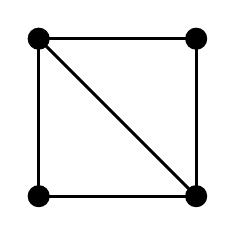
\begin{tikzpicture}[scale=1,looseness=1,auto,line width=.4mm]

      \draw (0,0) -- (0,2);
      \draw (0,2) -- (2,2);
      \draw (2,2) -- (2,0);
      \draw (2,0) -- (0,0);
      \draw (2,0) -- (0,2);

      \draw[fill=black] (0,0) circle(.12);
      \draw[fill=black] (0,2) circle(.12);
      \draw[fill=black] (2,2) circle(.12);
      \draw[fill=black] (2,0) circle(.12);

    \end{tikzpicture}
  \end{center}
\end{figure}
\vspace{-.5cm}

Combien d'arbres sous-tendants ce graphe possède-t-il?
\begin{solution}
\begin{align*}
    T(\begin{tikzpicture}
      \SetGraphUnit{0.3}
      \SetVertexNoLabel
      \Vertex[empty]{A}
      \NO[empty](A){D}
      \EA[empty](A){B}
      \NO[empty](B){C}
      \Edges(A,B,C,D,A,C)
    \end{tikzpicture}) & = T(\begin{tikzpicture}
      \SetGraphUnit{0.3}
      \SetVertexNoLabel
      \Vertex[empty]{A}
      \NO[empty](A){D}
      \EA[empty](A){B}
      \NO[empty](B){C}
      \Edges(A,B,C,D,A)
    \end{tikzpicture}) + T(\begin{tikzpicture}
      \SetGraphUnit{0.2}
      \SetVertexNoLabel
      \Vertex[empty]{A}
      \SOEA[empty](A){B}
      \SOEA[empty](B){C}
      \Edges[style={bend left}](A,B,C,B,A)
    \end{tikzpicture})\\
    & = T(\begin{tikzpicture}
      \SetGraphUnit{0.3}
      \SetVertexNoLabel
      \Vertex[empty]{A}
      \NO[empty](A){D}
      \EA[empty](A){B}
      \NO[empty](B){C}
      \Edges(D,A,B,C)
    \end{tikzpicture}) + T(\begin{tikzpicture}
      \SetGraphUnit{0.3}
      \SetVertexNoLabel
      \Vertex[empty]{A}
      \SOWE[empty](A){B}
      \SOEA[empty](A){C}
      \Edges(A,B,C,A)
    \end{tikzpicture}) + T(\begin{tikzpicture}
      \SetGraphUnit{0.2}
      \SetVertexNoLabel
      \Vertex[empty]{A}
      \SOEA[empty](A){B}
      \SOEA[empty](B){C}
      \Edges[style={bend left}](A,B,C,B)
    \end{tikzpicture}) + T(\begin{tikzpicture}
      \SetGraphUnit{0.3}
      \SetVertexNoLabel
      \Vertex[empty]{A}
      \SOEA[empty](A){B}
      \Edges[style={bend left}](A,B,A)
    \end{tikzpicture})\\
    & = 1 + T(\begin{tikzpicture}
      \SetGraphUnit{0.3}
      \SetVertexNoLabel
      \Vertex[empty]{A}
      \SOWE[empty](A){B}
      \SOEA[empty](A){C}
      \Edges(A,B,C)
    \end{tikzpicture}) + T(\begin{tikzpicture}
      \SetGraphUnit{0.3}
      \SetVertexNoLabel
      \Vertex[empty]{A}
      \SOEA[empty](A){B}
      \Edges[style={bend left}](A,B,A)
    \end{tikzpicture}) + T(\begin{tikzpicture}
      \SetGraphUnit{0.2}
      \SetVertexNoLabel
      \Vertex[empty]{A}
      \SOEA[empty](A){B}
      \SOEA[empty](B){C}
      \Edges[style={bend left}](A,B,C)
    \end{tikzpicture}) + T(\begin{tikzpicture}
      \SetGraphUnit{0.2}
      \SetVertexNoLabel
      \Vertex[empty]{A}
      \SOEA[empty](A){B}
      \SOEA[empty](B){C}
      \Edges[style={bend left}](A,B,C)
    \end{tikzpicture}) + T(\begin{tikzpicture}
      \SetGraphUnit{0.3}
      \SetVertexNoLabel
      \Vertex[empty]{A}
      \SOEA[empty](A){B}
      \Edges[style={bend left}](A,B)
    \end{tikzpicture}) + T(\begin{tikzpicture}
      \SetGraphUnit{0.3}
      \SetVertexNoLabel
      \Vertex[empty]{A}
      \SOEA[empty](A){B}
      \Edges[style={bend left}](A,B)
    \end{tikzpicture})\\
    & = 1 + 1 + 2 + 1 + 1 + 1 + 1\\
    & = 8.
  \end{align*}
\end{solution}
\subsection{Coupe et arbre sous-tendant}
Considérons le graphe connexe $G = (V, E, \psi)$. Etant donné une partition $\Pi = \{V_1, V_2\}$ de $V$, On définit la \emph{coupe} $C(\Pi)$ de $G$ relative à $\Pi$ comme l'ensemble des arêtes de $G$ suivant~:
\[
  C(\Pi) := \{ (v_1, v_2) \in E : v_1 \in V_1 \text{ et } v_2 \in V_2 \}.
\]
Montrez qu'une coupe et un arbre sous-tendant de $G$ ont au moins une arête en commun.
\begin{solution}
Si ils n'ont rien en commun, cela signifie que l'arbre n'est pas connexe car il y a une partition. Il y a, par conséquent, une contradiction.
\end{solution}
\subsection{Arbre de coup minimum}
Montrez que si on veut trouver un arbre de recouvrement qui minimise l'arête la plus chère, il suffit de trouver l'arbre de poids minimum.

\begin{solution}
Prenons par l'absurde qu'il existe un arbre de recouvrement $G$ qui minimise l'arête de plus grand poids et un arbre de recouvrement minimum $Q$ mais qui ne minimise pas l'arête de poids minimum. Cela signifie que certaines arêtes de $Q$ n'ont pas la valeur minimal. Dans ce cas, comme tout les noeuds sont atteint, il suffit de prendre les arêtes de poids inférieur dans $G$ et de remplacé c.
\end{solution}

\subsection{Graphe 3-connexe et 3-arête-connexe}
Trouvez un graphe 3-connexe et 3-arête-connexe.

\begin{solution}
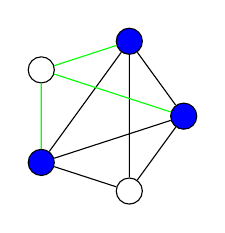
\begin{tikzpicture}
  % Define the points of a regular pentagon
  \path (0:1) node[draw,shape=circle,style={circle,fill=blue}] (P0) {};
  \path (1*72:1) node[draw,shape=circle,style={circle,fill=blue}] (P1) {};
  \path (2*72:1) node[draw,shape=circle] (P2) {};
  \path (3*72:1) node[draw,shape=circle,style={circle,fill=blue}] (P3) {};
  \path (4*72:1) node[draw,shape=circle] (P4) {};
  % Draw the edges of the pentagon
  \draw (P0) -- (P1) (P4) -- (P0) (P3) -- (P4) (P3) -- (P0) (P1) -- (P3) (P1) -- (P4);
  \draw[green] (P1) -- (P2) (P2) -- (P3) (P2) -- (P0); 
\end{tikzpicture}
\end{solution}

\subsection{$ \text{connectivité } \leq \text{ arête-connectivité } \leq \text{ degré minimum} $}
L'identité suivante a été vue au cours~:
\[
  \text{connectivité } \leq \text{ arête-connectivité } \leq \text{ degré minimum}
\]
Trouvez un graphe pour lequel les inégalités sont des égalités. Trouvez ensuite un graphe pour lequel les inégalités sont strictes.

\begin{solution}
Egalité : $3=3=3$
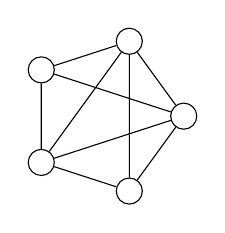
\begin{tikzpicture}
  % Define the points of a regular pentagon
  \path (0:1) node[draw,shape=circle] (P0) {};
  \path (1*72:1) node[draw,shape=circle] (P1) {};
  \path (2*72:1) node[draw,shape=circle] (P2) {};
  \path (3*72:1) node[draw,shape=circle] (P3) {};
  \path (4*72:1) node[draw,shape=circle] (P4) {};
  % Draw the edges of the pentagon
  \draw (P0) -- (P1) (P4) -- (P0) (P3) -- (P4) (P3) -- (P0) (P1) -- (P3) (P1) -- (P4) (P1) -- (P2) (P2) -- (P3) (P2) -- (P0); 
\end{tikzpicture}

inégalité : $1<2<3$
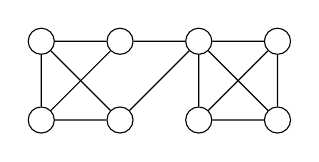
\begin{tikzpicture}
  % Define the points of a regular pentagon
  \path (0,0) node[draw,shape=circle] (P1) {};
  \path (0,1) node[draw,shape=circle] (P2) {};
  \path (1,0) node[draw,shape=circle] (P3) {};
  \path (1,1) node[draw,shape=circle] (P4) {};
  \path (2,0) node[draw,shape=circle] (P5) {};
  \path (2,1) node[draw,shape=circle] (P6) {};
  \path (3,0) node[draw,shape=circle] (P7) {};
  \path (3,1) node[draw,shape=circle] (P8) {};
  % Draw the edges of the pentagon
  \draw (P1) -- (P2) (P1) -- (P3) (P1) -- (P4) (P2) -- (P3) (P2) -- (P4) (P3) -- (P6) (P4) -- (P6) (P5) -- (P6) (P5) -- (P7) (P5) -- (P8) (P6) -- (P7) (P6) -- (P8) (P7) -- (P8); 
\end{tikzpicture}
\end{solution}

\subsection{Trouvez un graphe}
On définit $\delta$, $n$ et $k$ respectivement comme le degré minimum, le nombre de sommets et la connectivité d'un graphe simple $G$. Trouvez un graphe $G$ tel que $\delta = n-3$ et $k < \delta$.

\begin{solution}
$n=3$, $k=2$ (bleu) et $\delta = 3$
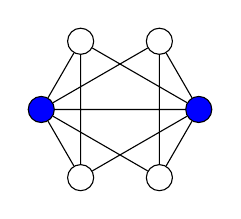
\begin{tikzpicture}
  % Define the points of a regular pentagon
  \path (0:1) node[draw,shape=circle,style={circle,fill=blue}] (P0) {};
  \path (1*60:1) node[draw,shape=circle] (P1) {};
  \path (2*60:1) node[draw,shape=circle] (P2) {};
  \path (3*60:1) node[draw,shape=circle,style={circle,fill=blue}] (P3) {};
  \path (4*60:1) node[draw,shape=circle] (P4) {};
  \path (5*60:1) node[draw,shape=circle] (P5) {};
  % Draw the edges of the pentagon
  \draw (P0) -- (P1) (P0) -- (P2) (P0) -- (P3) (P0) -- (P4) (P0) -- (P5) (P1) -- (P5) (P1) -- (P3) (P2) -- (P3) (P2) -- (P4) (P4) -- (P3) (P5) -- (P3);
\end{tikzpicture}
\end{solution}
